\documentclass{article}

%% Language and font encodings
\usepackage[english]{babel}
\usepackage[utf8x]{inputenc}
\usepackage[T1]{fontenc}

%% Sets page size and margins
\usepackage[a4paper,top=3cm,bottom=2cm,left=3cm,right=3cm,marginparwidth=1.75cm]{geometry}

%% Useful packages
\usepackage{amsmath}
\usepackage{float}
\usepackage{graphicx}
\usepackage[colorinlistoftodos]{todonotes}
\usepackage[colorlinks=true, allcolors=blue]{hyperref}

\title{CS 100 Assignment 1: Design}
\author{William Shiao, Siddhanth Sharma}

\begin{document}
\maketitle

\section{Introduction}

Our design is based around the Composite Pattern. Our RShell parses expressions into Commands and Connectors, which are then evaluated to generate the desired output.

\section{UML Diagram}

\begin{figure}[H]
\centering
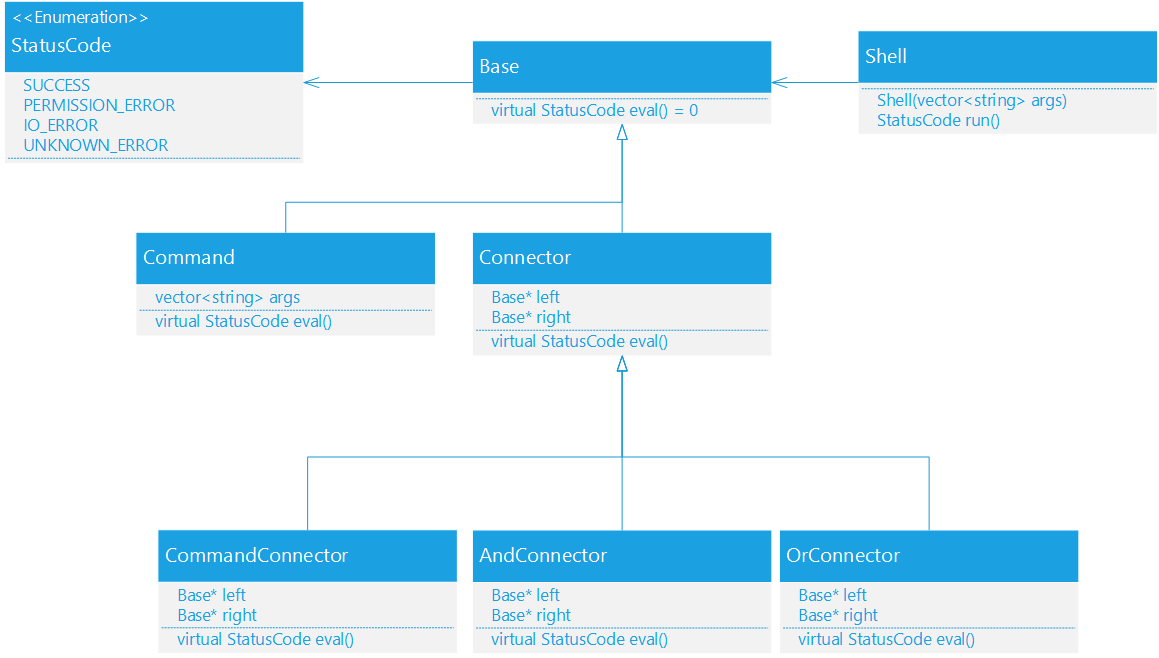
\includegraphics[width=1\textwidth]{uml.png}
\end{figure}

\section{Classes/Class Groups}

\subsection{Shell}

The \texttt{Shell} class is in charge of parsing user input and displaying the outputs. Its constructor also accepts arguments that can be used to change various settings.	

\subsection{StatusCode}

In the case of errors, we included the \texttt{StatusCode} enum so that the \texttt{Base::eval} and \texttt{Shell::run} functions can return the result of commands, which can then be use to display a more detailed error message to the user.

\subsection{Base}

\texttt{Base} is an abstract base class that is the parent of all classes except for \texttt{StatusCode} and \texttt{Shell}.

\subsection{Command}

A \texttt{Command} is any user input that is meant to execute a program. It has a member variable, \texttt{args}, that stores any arguments to be passed into the program.

\subsection{Connector}

The \texttt{Connector} class is used for operations that connect two user inputs. It stores the left and right sides of the connector as \texttt{Base} objects, which are then evaluated to generate the output.

\subsubsection{CommandConnector}

The \texttt{CommandConnector} (;) class allows the user to write multiple commands on a single line.

\subsubsection{AndConnector}

The \texttt{AndConnector} (\&\&) class allows the user to execute two commands, where the second command executes only after the first one succeeds.

\subsubsection{OrConnector}

The \texttt{OrConnector} (||) class allows the user to execute two commands, where the second command executes only after the first one fails.

\section{Coding Strategy}

We will collaborate via GitHub by working on separate branches and merging our changes after testing to assure proper functionality. We will also agree on a code formatting standard and use Kanban to manage workflow, with occasional physical meetings to reinforce understanding.

\section{Roadblocks}

Roadblocks that will most likely occur include: 

\begin{itemize}
\item Working at different speeds
\item Conflicting views on the progress of the project
\item Scheduling conflicts that could lead to unexpected errors regarding workflow
\item Miscommunication and/or misunderstanding during development
\end{itemize}
The majority of potential roadblocks can be solved with proper work ethics and communication. As long as we manage our workflow efficiently (most likely with the use of a Kanban board) and work around potential conflicts with our work, these roadblocks should be manageable.

\end{document}